\documentclass[12pt]{ruthesis}
%\documentclass[12pt]{amsart}
\usepackage{amsmath}
\usepackage{amssymb}
\usepackage{latexsym}
\usepackage{epsfig,epsf,rotating}
\usepackage{subfigure}
\usepackage{siunitx}
%\usepackage{pictex}
\usepackage{epsf}
\usepackage{theorem}
\usepackage{graphicx}
\usepackage{hyperref}
\usepackage{typedref}
\usepackage[version=3]{mhchem}
%\usepackage{cite}
\usepackage[numbers, sort&compress]{natbib}

\title{Microwave spectroscopy on two dimensional electron gas}
\ctitle{Microwave spectroscopy on two dimensional electron gas}
\author{Jie Zhang}
\department{Physics and Astronomy}
\school{Rice University}
\degree{Master of Science}

\committee {
		Rui-Rui Du\\
        Professor of Physics and Astronomy \and
        Junichiro Kono, Chair \\
        Professor of Electrical and Computer Engineering and Physics \& Astronomy \and
        Wei Li\\
        Associate Professor of Physics and Astronomy\and
       }

\address{Houston, Texas}
\donemonth{August} \doneyear{2015} \makeindex
\begin{document}

  \begin{frontmatter}
   \pagenumbering{roman}
   %\makecover
   \maketitle

\begin{abstract}

Microwave spectroscopy for detecting various resonance  of electrons is our main focus and we have been using electrical, thermal and absorption method for different purposes.

Electron Spin Resonance (ESR) and Cyclotron resonance (CR) are two of the most significant feature of electrons under magnetic field where electrical detection requires contacts on the sample which usually causes damages. In order to detect the electron spin resonance (ESR) of a single nano-object, high sensitive tool is required. So far, the best commercial ESR detector can detect around 1000 spins. We develop an ultra-sensitive calorimeter which is aimed at resolving the ESR of one nano-object. As a pretest, we show that CR can be measured via heat generated by resonant absorption of photons. An increase in the lattice temperature can be detected when the energy of the incident microwave photons matches the energy difference between adjacent Landau levels. They will be absorbed converting to phonons via non-radiative relaxation. A nano-calorimetry is constructed which can operate at 300 mK and precision of our thermometer is improved to tens of micro-Kelvins, thereby increasing the sensitivity to several nano-watts.

Edge state transport is also an interest of ours due to its pure one dimensionality and dissipationless feature. Microwave absorption spectroscopy of quantum droplet on two dimensional electron/hole gas is a powerful tool investigating the number and velocities of the charge modes. We have sample patterned with multiple circular dots on the order of several microns. It is directly placed onto the meander line superconducting waveguide positioned inside a resonance container. The whole setup is attached to the bottom of a top loaded Helium 3 cryostat with base temperature down to 300mK. This absence of quantum contact has the advantage over standard transport measurement with its high sensitivity and could be generalized to a common method probing edge states hosted in other new materials.


\end{abstract}

%\include{ack}
\tableofcontents
\listoffigures
%\listoftables
%   \include{ded}
\end{frontmatter}
\pagenumbering{arabic}
\linespacing{1.7}


\chapter{Introduction}\label{Intro}


\chapter{Transport behavior of electrons under the illumination of microwave}\label{Transport}

\section{SdH Oscillation and MIRO}\label{SdHO}
Shubnikov de Haas oscillations represents how longitudinal resistance of a Hallbar sample behaves in low magnetic field range. As soon as magnetic field is applied on a 2DEG system, the constant density of state immediately becomes isolated Dirac functions ideally with a spacing of $\hbar\omega_{c}$. ($\omega_{c}=\frac{eB}{m^{*}}$ is the cyclotron frequency) But the reality is they get broadened since the electrons can't avoid being scattered by other electrons, holes, phonons and impurities. These extended functions are the so-called Landau Levels with the same peak-peak spacing and a full width at half maximum being $\Gamma=\hbar/\tau q$. Here q is the quantum life time meaning the time span between two scattering events. In order to resolve the peak, one has to have sufficient magnetic field to meet the requirement $\hbar\omega_{x}>\Gamma$ which is equivalent to $\omega_{c}\tau q>1$. That means electron has to survive long enough to fulfill at least one cyclotron orbit without scattering. The total number of states in each Landau Level per unit area is marked by $n_{B}=\frac{eB}{h}$ giving a filling factor of $\mu =\frac{n_{2D}}{n_{B}}=\frac{h}{eB}n_{2D}$. Therefore, when the Fermi energy lies between two separate Landau Levels, longitudinal conductance reaches a local minimum and it gets to a local maximum when $E_{F}$ lies on the peak. As a function of magnetic field, the longitudinal resistance $R_{xx}$ represents oscillating behaviors which is known as Shubnikov de Haas oscillations. (Seen Figure 2.1)

\begin{figure}
  \centering
  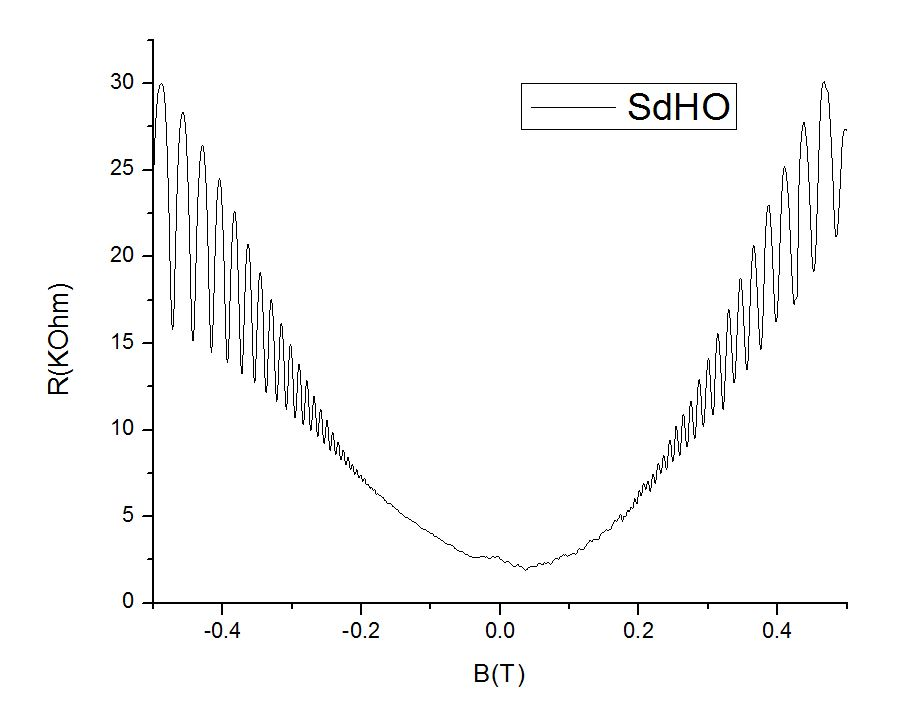
\includegraphics[totalheight=8cm]{figures/sdho.JPG}
  \caption{Shubnikov de Haas oscillations}
  \label{sdho}
\end{figure}


When microwave is applied, the figure changes quite dramatically . Additional maximums appear with different intensity at different harmonic peaks.

\begin{figure}
  \centering
  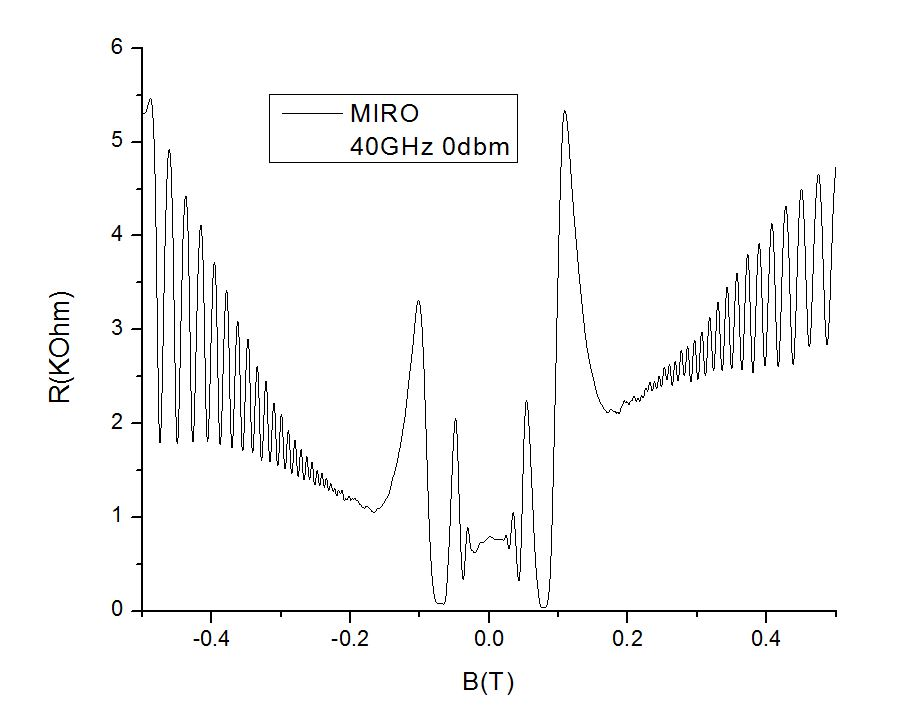
\includegraphics[totalheight=8cm]{figures/miro.JPG}
  \caption{MIRO}
  \label{miro}
\end{figure}
 





\section{Zero Resistance State}\label{ZRS}










\chapter{Thermal detection on behavior of electrons under the illumination of microwave}\label{Thermal}





\section{Theoretical Support}\label{Theoretical}

\begin{figure}
  \centering
  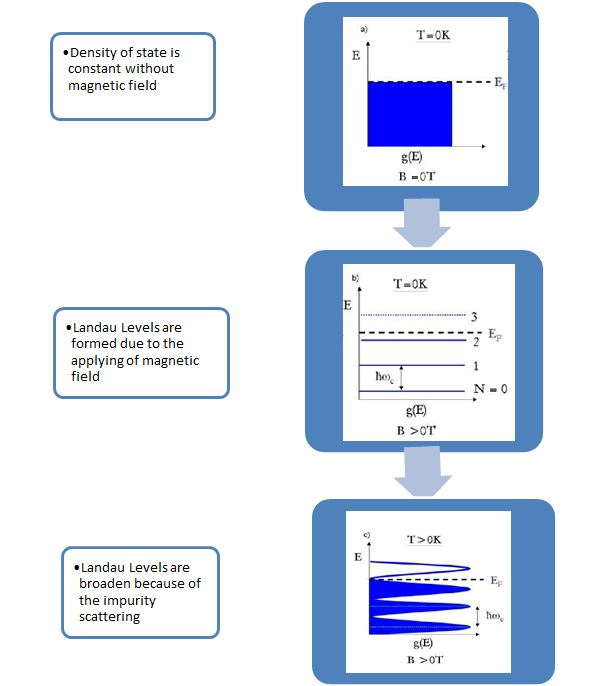
\includegraphics[totalheight=8cm]{figures/llformation.JPG}
  \caption{formation of Landau Levels}
  \label{llformation}
\end{figure}
 
\begin{figure}
  \centering
  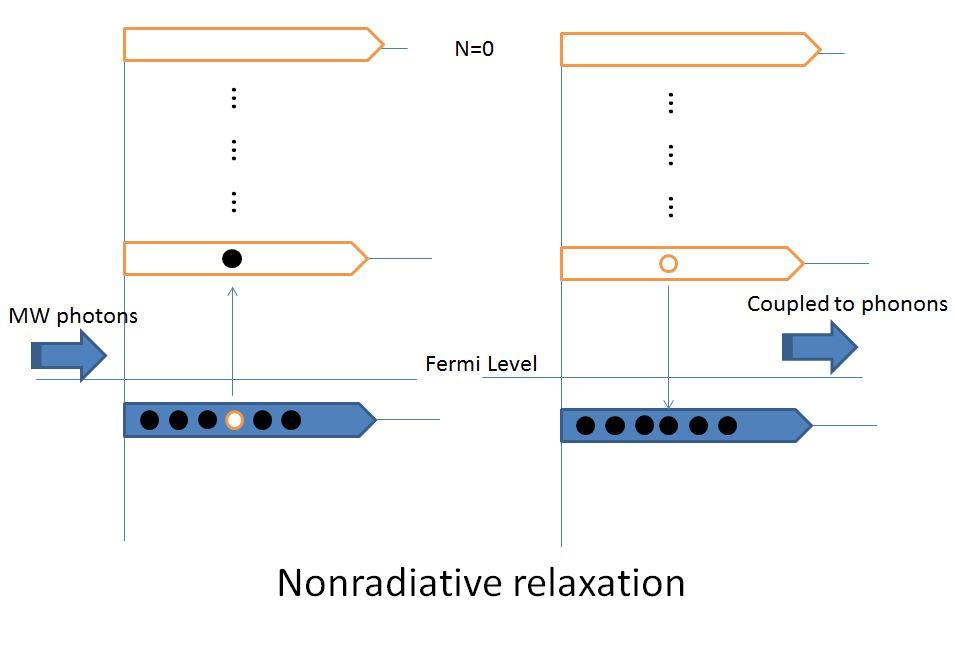
\includegraphics[totalheight=8cm]{figures/nonradiative.JPG}
  \caption{Non-radiative relaxation}
  \label{nonradiative}
\end{figure}
 
 
 
 
 
 
\section{Setup Construction}\label{Construction}

\begin{figure}
  \centering
  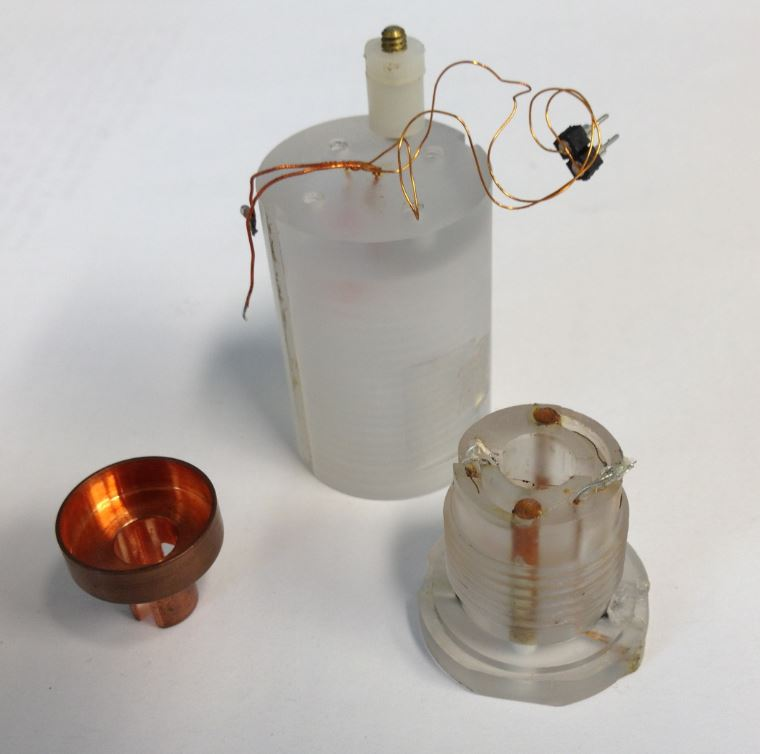
\includegraphics[totalheight=8cm]{figures/vacumcan.JPG}
  \caption{1266 Epoxy vacum can}
  \label{vacum-can}
\end{figure}
 
 
\begin{figure}
  \centering
  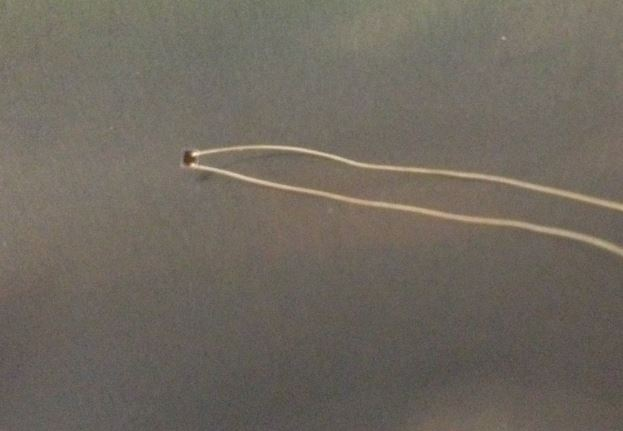
\includegraphics[totalheight=8cm]{figures/thermometercx.JPG}
  \caption{Cernox thermometer}
  \label{thermometer}
\end{figure}
 

\begin{figure}
  \centering
  \includegraphics[totalheight=8cm]{figures/SCHEMA.JPG}
  \caption{Thermal detection setup schema}
  \label{thermal-schema}
\end{figure}
 
 
\begin{figure}
  \centering
  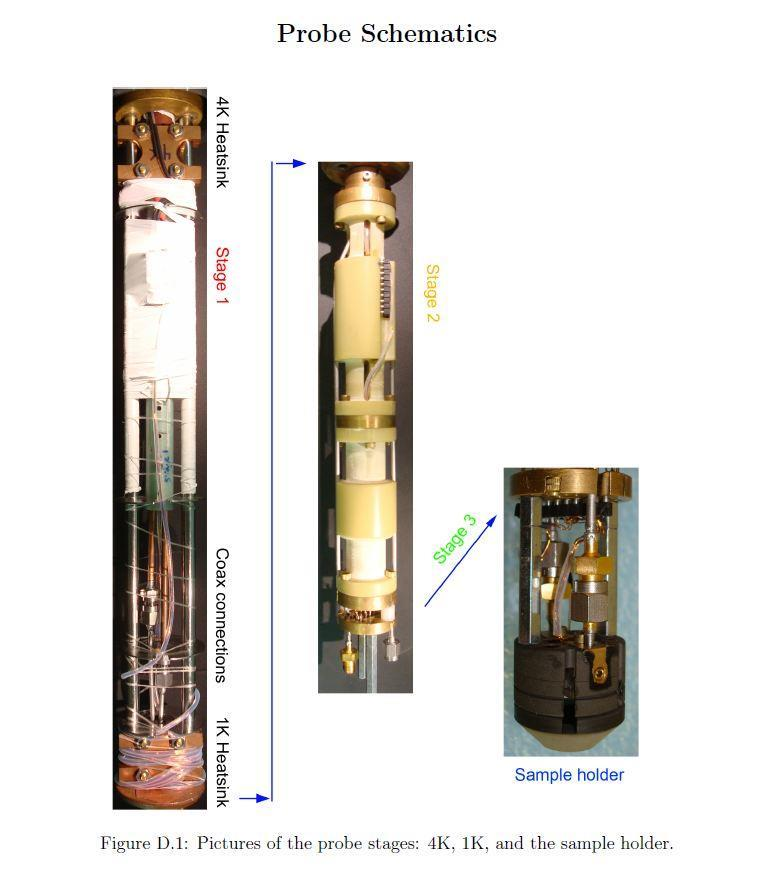
\includegraphics[totalheight=8cm]{figures/probe.JPG}
  \caption{He3 top loaded Refridgerator coaxial probe}
  \label{probe}
\end{figure}
 
 
 
 
 
 


\section{Cyclotron Resonance Pretest}\label{Cyclotron}

\begin{figure}
  \centering
  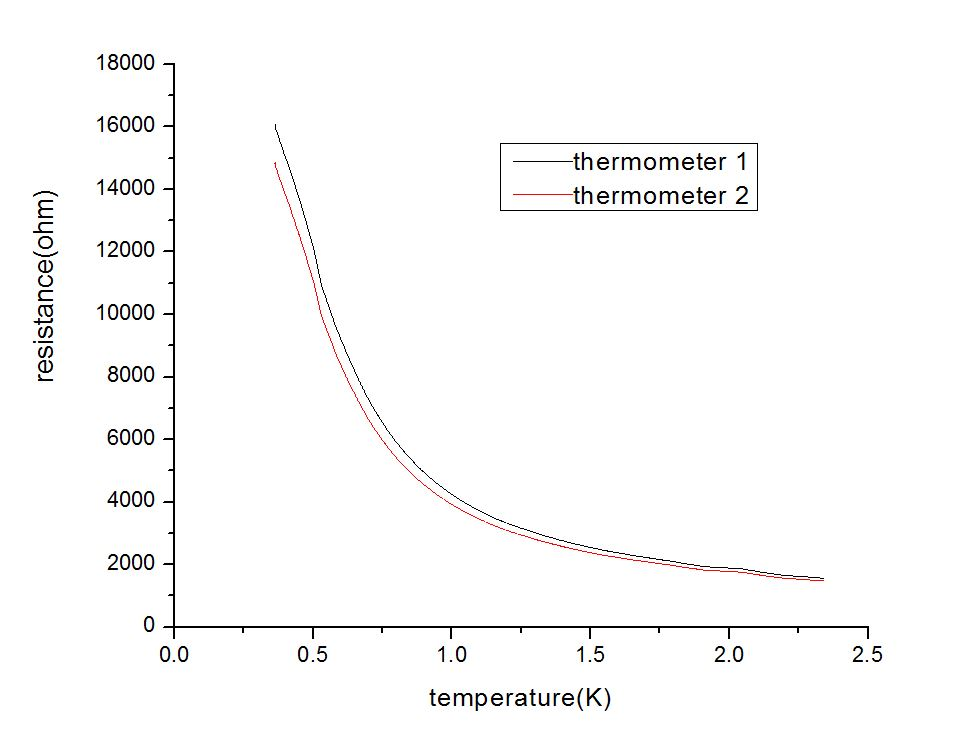
\includegraphics[totalheight=8cm]{figures/R(T).JPG}
  \caption{Temperature dependence of the thermometers}
  \label{r(t)}
\end{figure}
 
 
\begin{figure}
  \centering
  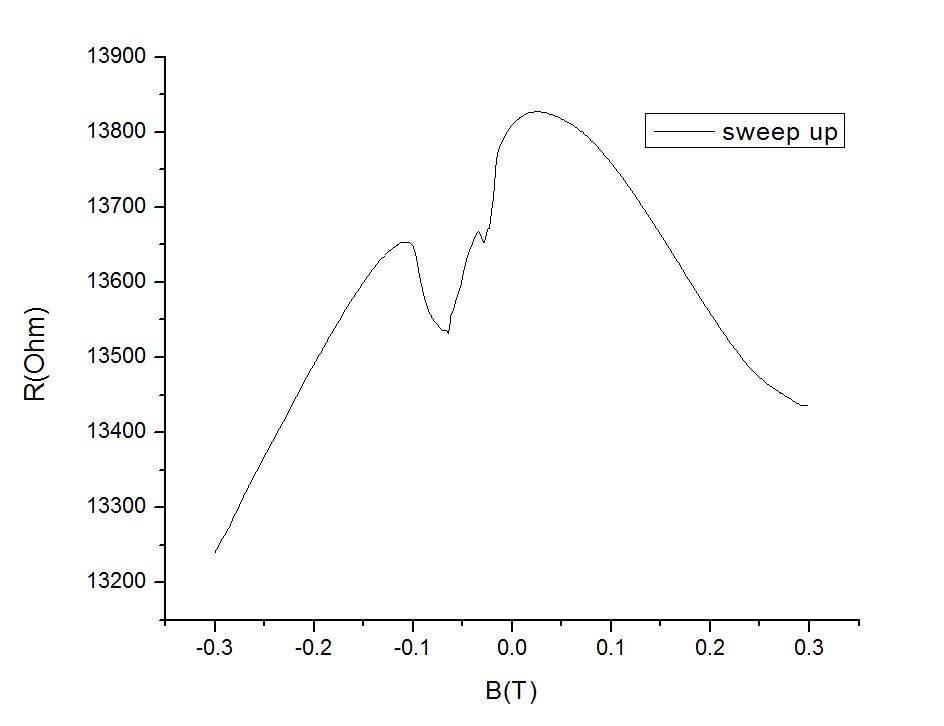
\includegraphics[totalheight=8cm]{figures/R(B)UP.JPG}
  \caption{Background sweeping}
  \label{r(b)}
\end{figure}

\begin{figure}
  \centering
  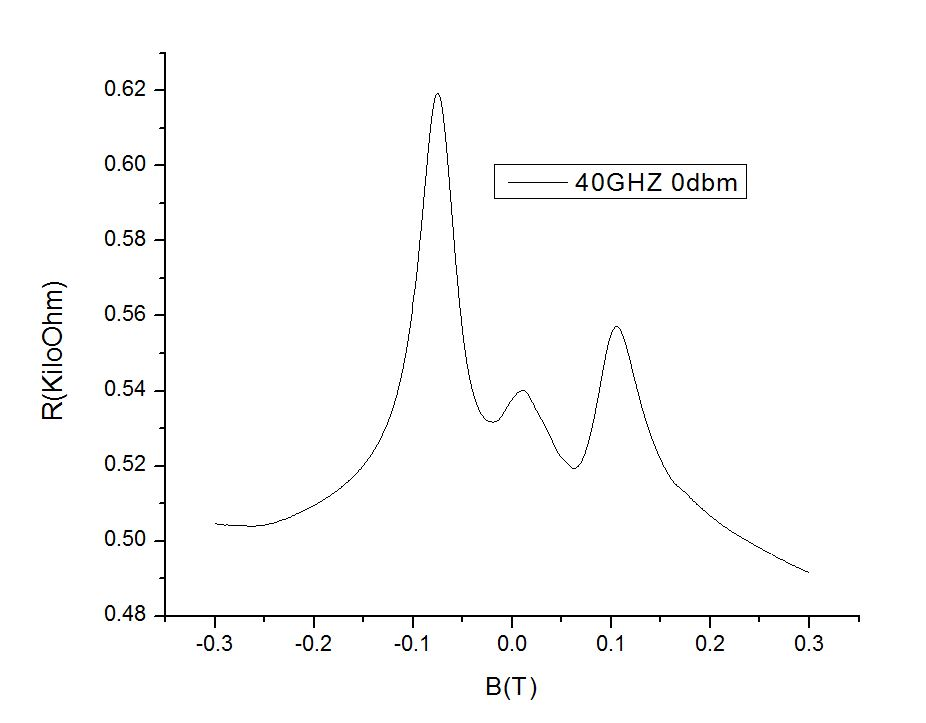
\includegraphics[totalheight=8cm]{figures/0dbm.JPG}
  \caption{CR at 0dbm 40GHz}
  \label{0dbm_40ghz}
\end{figure}
 
 
\begin{figure}
  \centering
  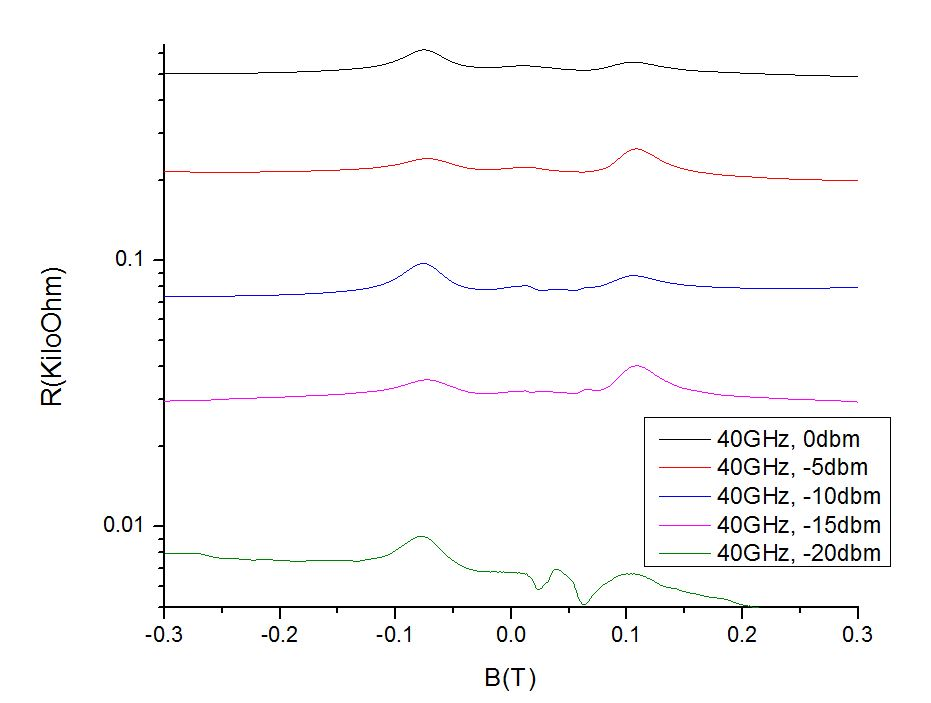
\includegraphics[totalheight=8cm]{figures/thermopowerdep.JPG}
  \caption{Power dependence}
  \label{thermopowerdep}
\end{figure}
 






\section{Spin Resonance on DPPH}\label{DPPH}


\begin{figure}
  \centering
  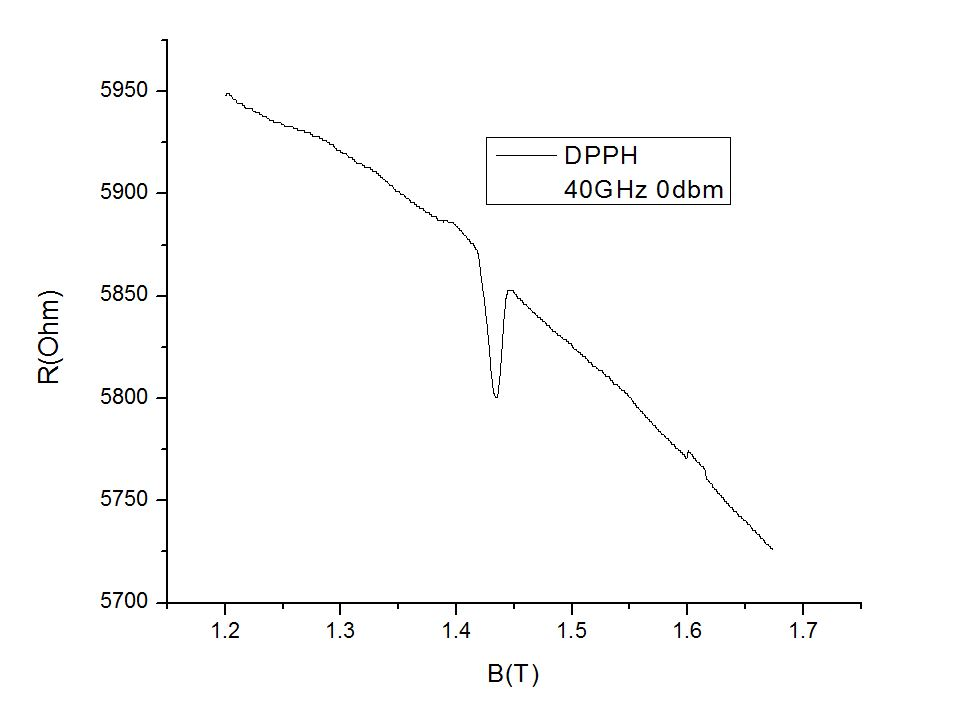
\includegraphics[totalheight=8cm]{figures/dpph_esr.JPG}
  \caption{ESR of DPPH}
  \label{dpph_esr}
\end{figure}
 
 
\begin{figure}
  \centering
  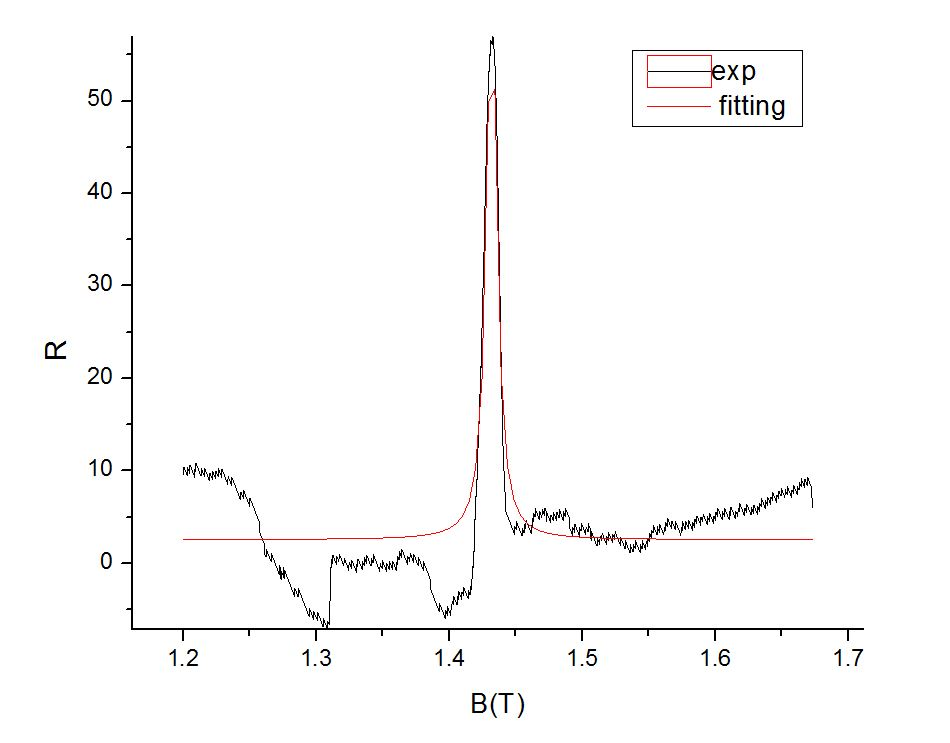
\includegraphics[totalheight=8cm]{figures/dpph_fitting.JPG}
  \caption{ESR Fitting of DPPH}
  \label{dpph_fitting}
\end{figure}
 









\chapter{Microwave absorption spectroscopy of electrons in 2DEG}\label{Absorption}




\section{Setup Construction}\label{Construction}

\begin{figure}
  \centering
  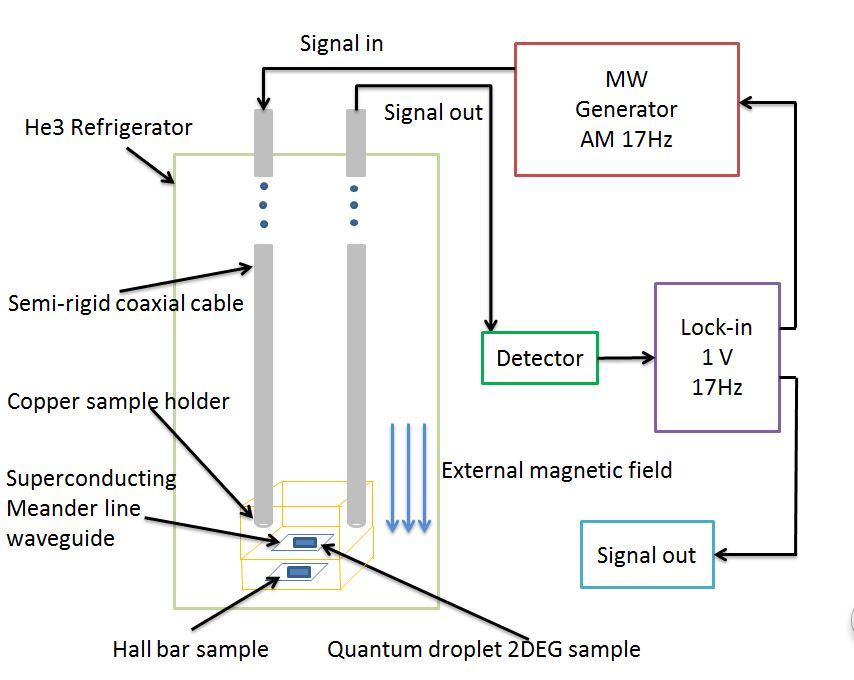
\includegraphics[totalheight=8cm]{figures/configuration.JPG}
  \caption{Microwave absorption spectroscopy construction}
  \label{configuration}
\end{figure}
 
 
 
 
 
 
 

\section{Cyclotron Resonance Pretest}\label{Cyclotron}

\begin{figure}
  \centering
  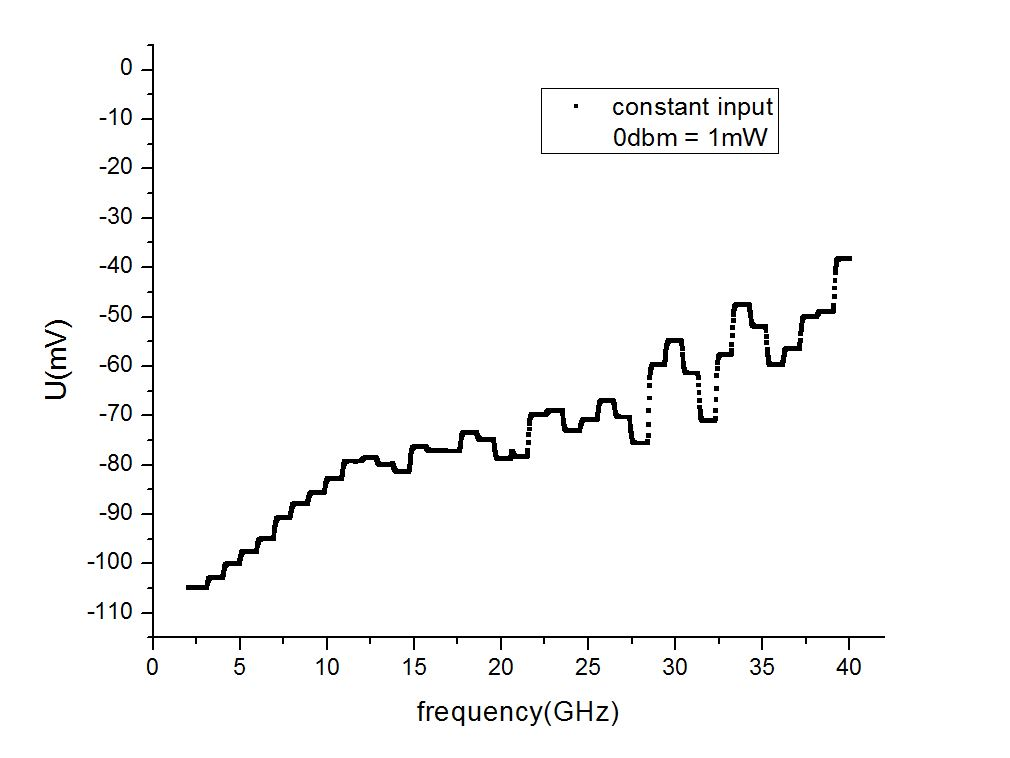
\includegraphics[totalheight=8cm]{figures/spec.JPG}
  \caption{setup calibration 1}
  \label{spec}
\end{figure}
 

\begin{figure}
  \centering
  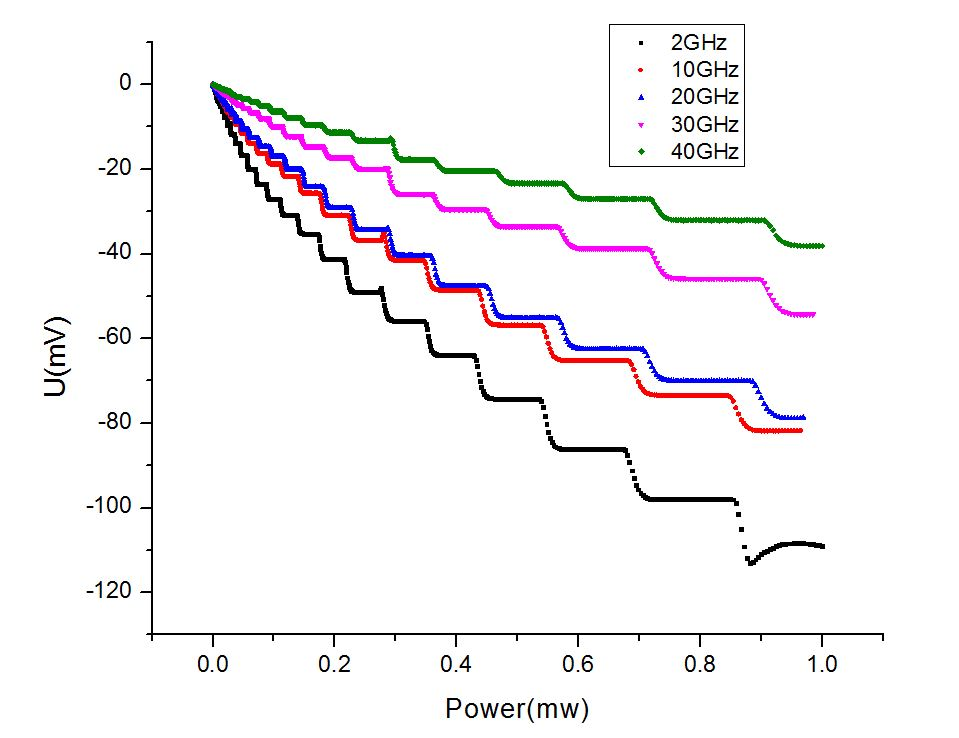
\includegraphics[totalheight=8cm]{figures/multifre.JPG}
  \caption{setup calibration 2}
  \label{multifre}
\end{figure}
 

\begin{figure}
  \centering
  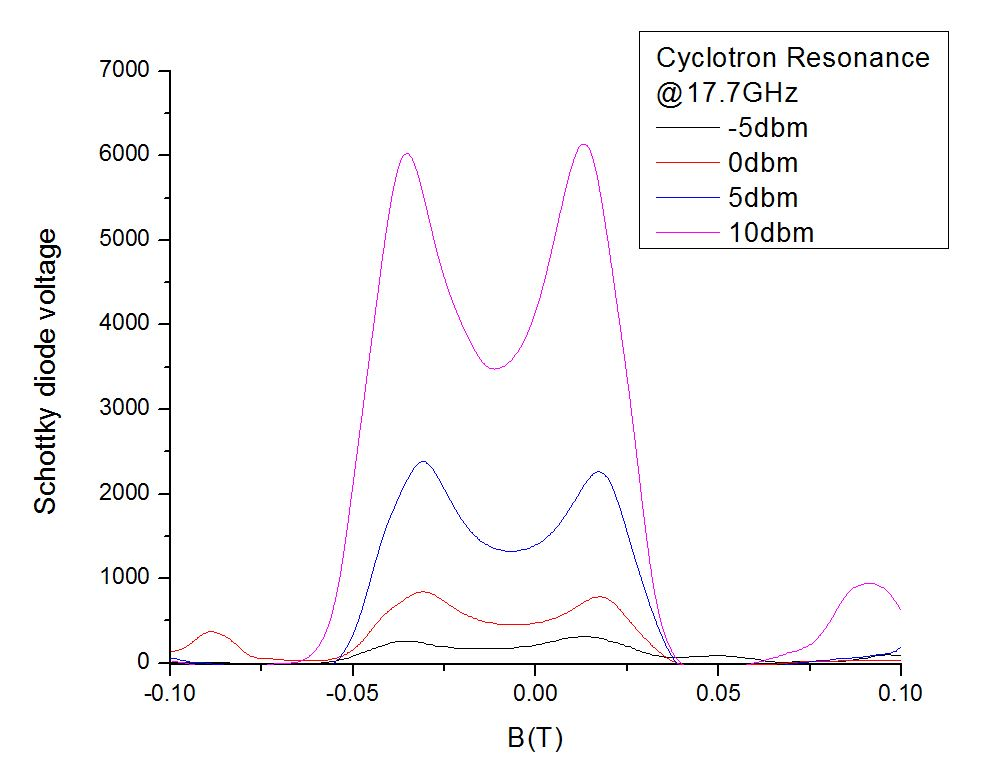
\includegraphics[totalheight=8cm]{figures/CRpowerdep.JPG}
  \caption{cyclotron pretest}
  \label{crpowerdep}
\end{figure}
 







\section{Improvement underway}\label{Improvement}








\cite{Chen01APL}.
\figureref{Conductance}.






\chapter{Summary}\label{summary}





\appendix

%\include{append-a}
%\appendix
%\addcontentsline{toc} {chapter}{\numberline {}Appendix A}
%\include{append-a}
%\include{append-b}
%\addcontentsline{toc} {chapter}{\numberline {}Bibliography}{}
%\include{biblio}

\bibliographystyle{ieeetr}
\bibliography{Jie Zhang}
\end{document}
